
\subsection{Punto \textbf{3}}

\begin{itemize}
\item \emph{\textbf{Realizar el diseño físico (layout) del inversor utilizando el programa Synopsys. Verificar DRC y LVS. Incluir una captura de pantalla incluyendo una regla que permita verificar los $W$ de los transistores.}}
\end{itemize}


En la figura~\figref{fig:fig_inverter_layout} puede verse el layout diseñado, y pueden verse las reglas que permiten apreciar el pitch y el W de los transistores. Y en la figura~\figref{fig:fig_inverter_load_layout} puede de la misma forma verse el layout del inversor mínimo diseñado. Ambos layouts fueron verificados exitosamente con \textbf{DRC} y \textbf{LVS}.



\begin{figure}[H] %htb
\begin{center}
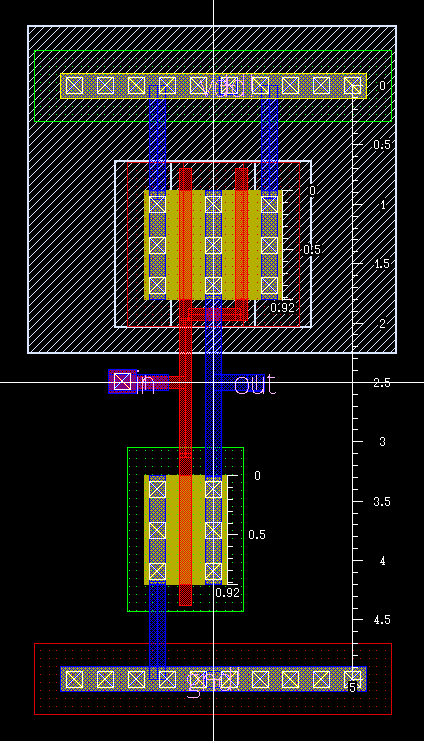
\includegraphics[width=0.45 \textwidth, angle=0]{./img/point3/TEST_LOGIC_GATES_Inverter_layout}
\caption{\label{fig:fig_inverter_layout}\footnotesize{Inversor \textbf{CMOS} diseñado (layout).}}
\end{center}
\end{figure}

\vfill
\clearpage


\begin{figure}[H] %htb
\begin{center}
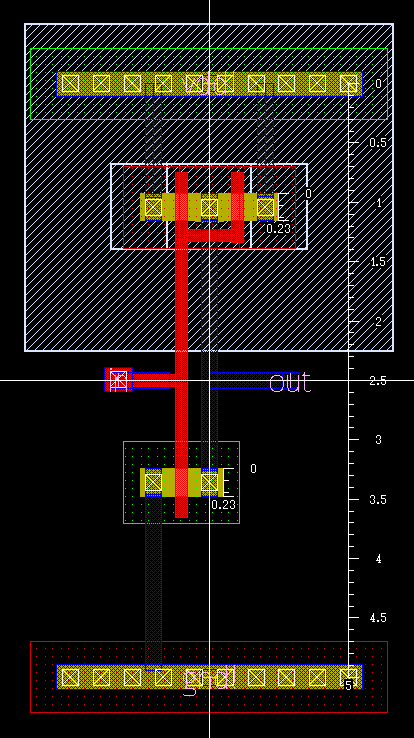
\includegraphics[width=0.45 \textwidth, angle=0]{./img/point3/TEST_LOGIC_GATES_Inverter_load_layout}
\caption{\label{fig:fig_inverter_load_layout}\footnotesize{Inversor \textbf{CMOS} mínimo diseñado (layout).}}
\end{center}
\end{figure}

\vfill
\clearpage